\documentclass[twocolumn]{article}
	\usepackage[
	top    = 2.8 cm,
	bottom =  2.8 cm]{geometry}

	\usepackage{hyperref}

	\usepackage{graphicx}  % needed for figures
	\usepackage{dcolumn}   % needed for some tables
	\usepackage{bm}        % for math
	\usepackage{amssymb}   % for math
	\usepackage{amsmath}
	\usepackage{nameref}
	\newcommand{\degree}{\ensuremath{^\circ}}
	\def\mean#1{\left< #1 \right>}
	%%% make INLINE SUBSECTIONS 
		
		% 1em is in the 'sep' slot, which controls how much space is between the numbering and the section heading text. 1em is equal to the width of 1 times the width of a capital 'M' in font you're using. 
	\usepackage{titlesec}
	\titleformat{\subsection}[runin]
	{\normalfont\large\bfseries}{\thesubsection}{1em}{}
		% The formatting settings above other than the 'runin' option are the default settings for subsections. 


	\begin{document}
	\title{Problem set }
	\author{Giulio Ungaretti}
	\date{\today}
	\twocolumn[
	   \begin{@twocolumnfalse}
	     \maketitle
	     \begin{abstract}
	       Problem set solutions.
	     \end{abstract}
	     \tableofcontents
	   \end{@twocolumnfalse}
	  ]

\clearpage
\section{Distributions \& \\ probabilities} % (fold)
	\label{sec:Distributions and probabilities}
	\subsection{} % (fold)
	\label{sub:}
	% subsection  (end)
	Given the PDF:
	\begin{equation}
		\operatorname{f}{\left (t \right )} = C e^{- \frac{t}{\tau}}
	\end{equation}
	in the range $t$ $\in~$[$ t_0, \infty $], the value of C for which the PDF is normalized is:

	\begin{equation}
		\int_{t_{{0}}}^{\infty} C e^{- \frac{t}{\tau}}\, dt = 1 \longrightarrow C =  \frac{
		e^{
		\frac{t_0}{\tau}
		}}
		{\tau}
	\end{equation}
	I note a close resemblance of our PDF to the exponential distribution, and they coincide if $t_0 = 0$. 
	The mean, or better, the expectation  value is then:
	\begin{equation}
	\mathbb{E} [t] = \int_{t_0}^{\infty} t \operatorname{f}{(t) d t } \longrightarrow  t_0 + \tau
	\end{equation}
	It's nice to note that for $t_0 = 0$ it matches the well known result for the exponential distribution.
	The width could be quantified with the variance as:
	\begin{multline}
		Var(t) = \mathbb{E}[x^2] - (\mathbb{E}[x])^2 = \\
		= 
		\int_{t_0}^{\infty} t^2 \operatorname{f}{(t) d t } 
		-(\int_{t_0}^{\infty} t \operatorname{f}{(t) d t })^2 = \\
		= 2 \tau ^ 2 + 2 t_o \tau +t_0 ^2  - ( t_0 + \tau ) ^ 2 = \\
		= \tau ^ 2
	\end{multline}
	A graphical representation of all said above is found in Figure~\ref{fig:pdf}.
	\begin{figure}[h!]
		\begin{center}
			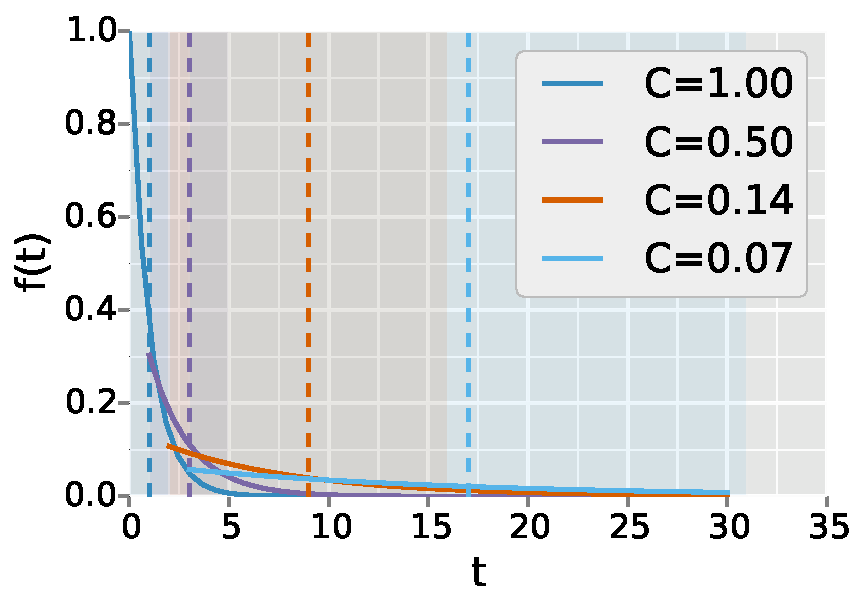
\includegraphics[width= 0.4 \textwidth]{fig/graph.pdf}
		\end{center}
		\caption{Plot of the given PDF, for different values of $ \tau $ and $t_0 $. Dashed lines are the calculated expectation values, and the shaded area represent plus and minus one square root of the variance around the mean.}
		\label{fig:pdf}
	\end{figure}



	\subsection{} % (fold)
	\label{sub:}
	Assuming that little Peter is a fair pal, and is using fair coins then the probability of success (heads) follows the binomial distribution.
	If we call $n$ the number of tries, $p= \frac{1}{2}$ the probability for each event to success, and $r$ the number of success out of $n$ tries, the probability is the following: 
	\begin{multline}
	\label{eq:bin}
		P (n,r) = \frac{n!}{r!(n-r)!} p ^ r (1-p)^{n-r} \\ 
		 = \tbinom n r p ^ r (1-p)^{n-r}
	\end{multline}
	The \emph{chance} of getting 14 or more heads with 20 coin flips is \emph{low}, as it is possible to see in~Figure~\ref{fig:lil}. The probability of getting more than 14 heads is calculated summing equation~\ref{eq:bin} for r going from 14 to 20.
	The probability is  $\approx 5 \% $.

	\begin{figure}[h]
		\begin{center}
			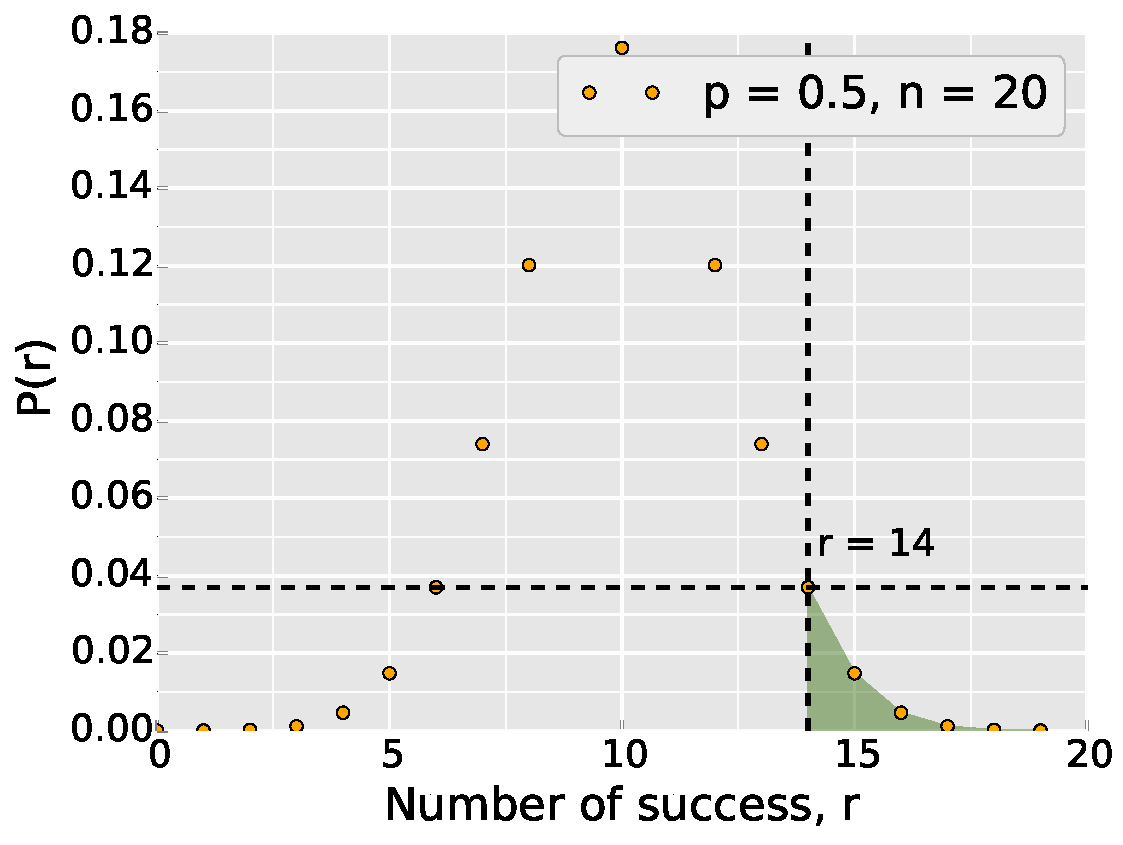
\includegraphics[width=.45 \textwidth]{fig/lil.pdf}
		\end{center}
		\caption{Probability of coin flips. The parameters are reported in the legend; the shadowed area quantifies the chance of getting 14 or more heads.}
		\label{fig:lil}
	\end{figure}


	To find the chance that little Peter gets at least 18 coin at once when flipping 20 coins 100 times, first the probability $P_{18}$ is calculated summing equation \ref{eq:bin} using $p= \frac{1}{2}$, $n=20$, and $r=[18,20]$.
	It is easy to see that the distribution of the chances of getting at least 18 successes is still binomial but with p = $P_{18}$, $n=100$, and $r=1$.
	The probability of getting one time a success is: $P(1) \approx 0.0002$. The chance of getting more than one is quantified as said before and it is  $\approx 2 \% $.
% subsection  (end)
% section Distributions and probabilities (end)
\clearpage
\section{Error propagation} % (fold)
\label{sec:error_propagation}
\subsection{} % sub:gravity (fold)
	Three different ways are employed to calculate the average of the given measurements, namely the arithmetic mean, a error weighted mean and finally a fit with a zeroth order polynomial.
	The last two options require to accept and believe in the reported experimental errors.
	The results are reported in Figure~\ref{fig:g}.

	\begin{figure}[h!]
		\begin{center}
			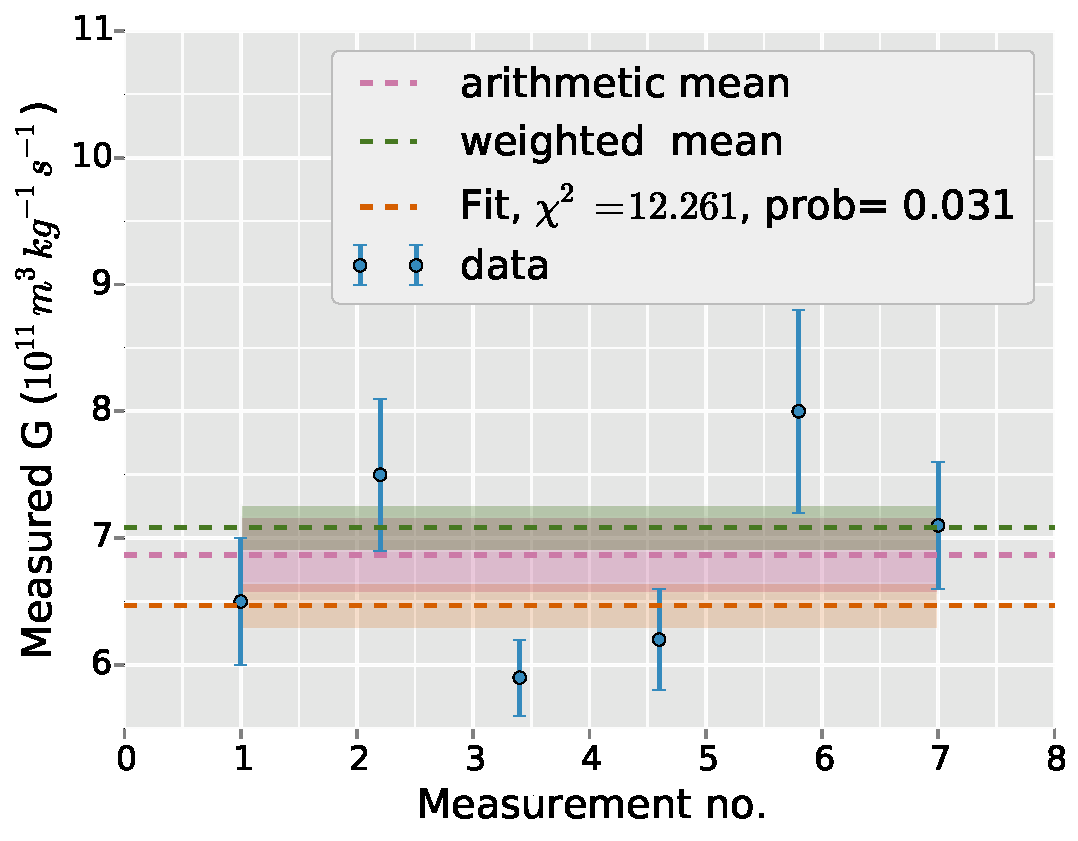
\includegraphics[width=.4\textwidth]{fig/g.pdf}
		\end{center}
		\caption{Graphical presentation of the given measurements and three differently calculated averages. The shadowed areas around each average value are plus and minus $\sigma_{\mu}$, the associated error.}
		\label{fig:g}
	\end{figure}

	The $\chi ^2 $ probability density function is reported in Figure~\ref{fig:xpdf} along with the probability of getting the same $\chi ^2 $ found in the aforementioned zeroth order polynomial fit.

	\begin{figure}[h!]
		\begin{center}
			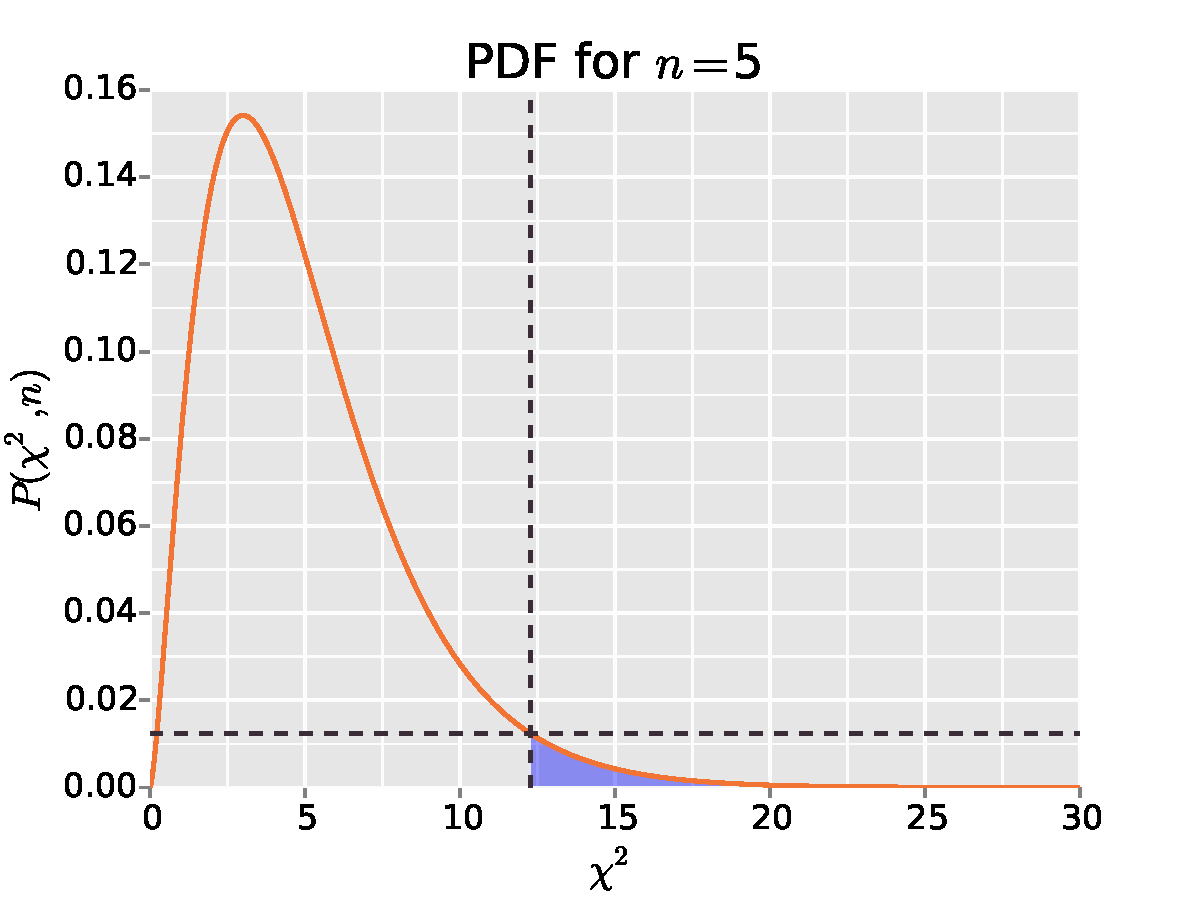
\includegraphics[width=.4 \textwidth]{fig/xpdf.pdf}
		\end{center}
		\caption{$\chi^2$ distribution for five degrees of freedom. Shaded area represent the probability of obtaining a $\chi^2$ greater the one obtained for the fit reported in Figure~\ref{fig:g}.}
		\label{fig:xpdf}
	\end{figure}
	The result obtained are summarized in Table~\ref{tab:res}.

	\begin{table}[htpb]
		\caption{Results. The averages and their errors are reported in units of: $10^{-11} m^3 kg^{-1} s^{-2}$.}
		\label{tab:res}
		\begin{center}
			\begin{tabular}{l|ccc}
			\hline

			\hline
			\textbf{method} & \textbf{average} & \textbf{uncertainty} & \textbf{$\chi ^2 $(prob)} \\
			\hline
			fit & 6.5 & .2 & 12.261 (0.031) \\
			$<G> $ & 6.9 & .3 & - \\
			$<G>_W$ &  7.1 & .2 & - \\
			\hline
			\hline
			\end{tabular}
		\end{center}
	\end{table}

	% section error_propagation (end)
	As it possible to see the fit is the method that is better representing the data with an average value.
	Moreover it is also compatible with the \emph{true} value of G ($ G = 6.6738 \pm .0008  \times 10^{-11} \ \mbox{m}^3 \ \mbox{kg}^{-1} \ \mbox{s}^{-2} $).
	The probability of the fit is not particularity high but is expected due to the low number of measurements.
	Lastly it is possible to note that the probability to get $\chi ^2 \gtrsim 12.261 $ is $ \approx 3 \% $ according the the $\chi ^2$ distribution (Figure~\ref{fig:xpdf}, shaded area).
\subsection{} % (fold)
\label{sub:gridiron}
	The uncertainty on a time measurement with a gridiron pendulum is:
	\begin{equation}
		\sigma_t  = 2 \pi \sqrt{ (\frac{1}{2 \sqrt{g L }} ) ^{2} \sigma_L ^2 +
		\sigma_g ^2 (\frac{\sqrt{L}}{2} g^{-\frac{3}{2}})^2
		}
	\end{equation}
	where L is the length of the pendulum, g is the gravitational constant with an error $\sigma_g$.
	If one considers that the error on the measurement on the length is \textbf{only} related to the thermal expansion of the materials making the pendulum then $\sigma_L$ can be calculated as:
	\begin{equation}
		\sigma_L = \sum_i \alpha_i  \Delta T  L_i
	\end{equation}
	where $\alpha_i$ is the linear coefficient of expansion for the \emph{ith} material, $L_i$ its length and $\Delta T $ the temperature fluctuation of the system.

	If the pendulum is made of a single component:
	\begin{equation}
	\sigma_t  = \pi \sqrt{L \left(\frac{\Delta T^{2} \left(a_{1} \right)^{2}}{g} + \frac{\sigma_{g}^{2}}{g^{3}}\right)}
	\end{equation}
	whereas if the pendulum is made of two components with a length ratio of $\lambda$:
	\begin{equation}
	\sigma_t  = \pi \sqrt{L \left(\frac{ \Delta  T^{2} \left(a_{1} - a_{2} \lambda \right)^{2}}{g} + \frac{\sigma_{g}^{2}}{g^{3}}\right)}
	\end{equation}

	It's easy to see that the error coming from the thermal expansion can be killed by choosing the correct material combination such that $ \left(a_{1} - a_{2} \lambda\right) \approx 0 $. Strangely enough that's the case for the iron/brass combo.
	% subsection  (end)
\subsection{} % (fold)
\label{sub:snell}
	To calculate the index of refraction (IOR) of a solution ($n_{sol}$) with respect to air one has to rearrange Snell's law and to calculate the error ($\sigma_{n_{sol}}$) one has to consider the IOR of air a value ($n_{air} =1 $) without error.
	\begin{equation}
	n_{sol} = \frac{ sin(\theta_{air})}{sin(\theta_{sol})} 
	\end{equation}

	\begin{multline}
	\sigma_{n_{sol}} = (\left[\frac{cos(\theta_{air})}{sin(\theta_{sol})}  \sigma_{air} \right]^2 + \\
	+ \left[ \frac{2 cos(\theta_{sol})}{1+cos(\theta_{sol})-1}  sin(\theta_{air}) \sigma_{sol}  \right] ^2 )^{\frac{1}{2}}
	\end{multline} 
	To determine the percentage and its error of sugar in the solution, using two known and error-less standard $n_1 = 1.3330$, and $n_2 = 1.4774$ for a  0\% and a 75\% solution respectively one has to use the following equations:
	\begin{equation}
	\% sugar = ( n_{sol} - 1.3330) \frac{75}{ (1.4774- 1.3330)}
	\end{equation}
	\begin{equation}
		\sigma_{\%} = \frac{75}{ (1.4774- 1.3330)} \sigma_{n_{sol}}
	\end{equation}
	The results are reported in Table~\ref{tab:snell}.
	\begin{table}[h!]
		\caption{Snell's law results}
		\label{tab:snell}
		\begin{center}
			\begin{tabular}{l|cc}
			\hline

			\hline
			\textbf{} & \textbf {$n_{sol}$ } & \textbf{ \% sugar} \\
			\hline
				value & 1.385  & 27 \\
				error & 0.008 & 4 \\
			\hline

			\hline
			\end{tabular}
		\end{center}
	\end{table}
	% subsection  (end)

\section{Monte Carlo} % (fold)
\label{sec:monte_carlo}
\subsection{}
 Having a PDF:
 \begin{equation}
 \label{eq:mcpdf}
 	\operatorname{f}{\left (x \right )} = \frac{C}{x^{3}}
 \end{equation}
 normalized for the value of $C=2$.
 We want to generate numbers that follow this PDF. 
 The transformation method would  work as the integral of the PDF:
 \begin{multline}
 	\int_{1}^{x(r)} \frac{2}{x^{3}}\, dx = 1 - \frac{1}{x(r)^{2}} = r
 \end{multline}
	is  invertible, given that $r \in [0,1[$. 
	A thousand number according to the transformation method are calculated and they are reported in 

	\begin{figure}[h!]
		\begin{center}
			\includegraphics[width = .4 \textwidth]{fig/monteCPDF}
		\end{center}
		\caption{One thousand number following the PDF reported in equation \ref{eq:mcpdf},generated via a Montecarlo Method.}
		\label{fig:figure1}
	\end{figure}


\subsection{}

	The mean of a particular outcome for $n$ dice is given by: 

	\begin{eqnarray}
	\mu_{i} &=& n \frac{1}{s}
	\end{eqnarray}

	where $ s $ is the number of the sides of that particular dice. The mean of the sum is just the sum of the means so 

	\begin{eqnarray}
	\mu_{\sum} &=& \frac{\sum\limits_{i}^{s}i}{s}
	\end{eqnarray}

	For the different dice, the mean of the sum is again the sum of the means, so : 


	\begin{eqnarray}
	\mu_{\sum\sum} &=& \frac{10\sum\limits_{i=1}^{6}i}{6} +\frac{6\sum\limits_{i=1}^{8}i}{8}+\frac{3\sum\limits_{i=1}^{10}i}{10}\\
	&=& 16.5+27+35\\
	&=& 78.5
	\end{eqnarray}


	The variance of each possible outcome of a dice is a binomially distributed random variable, thus the variance is just like for a binomial distribution with number of tries $n$ : 

	\begin{eqnarray}
	\sigma^{2}&=& n p_{i}(1-p_{i})
	\end{eqnarray}

	The variance for the sum is in this case just the sum of the variances, since every dice is independent: 

	\begin{eqnarray}
	\sigma^{2} &=& \mu_{1}\frac{9}{10} + \mu_{2}\frac{7}{8} + \mu_{3}\frac{5}{6}\\
	\rightarrow \sigma &=& 8.2 
	\end{eqnarray}
    Assuming the sum to follow a Gaussian distribution  the prob of having a sum $\ge$ 100 is~$\approx 2.6$ sigma away which means a probability of~$\approx~0.37~\%$.

    Using a Monte Carlo (MC) simulation the chance of getting a sum $\ge$ 100 is estimated for different number of runs. It expected that increasing  the
    number of runs will increase the probability as the distribution turn more and more into a Gaussian.
    The results of the MC simulation are reported in Figure~\ref{fig:figure1}.
    \begin{figure}[h]
    	\begin{center}
    		\includegraphics[width = .5 \textwidth]{fig/histplotdices.pdf}
    	\end{center}
    	\caption{MC simulation of the sum of  10-sided, 6 8-sided, and 10 6-sided dice.}
    	\label{fig:figure1}
    \end{figure}

    For 10, 100, 10000, 100000 runs the probability is 0\%,0\%, 0.01\%, 0.04 \% respectively.
% section monte_carlo (end)

\section{Statistical tests} % (fold)
\label{sec:statistical_tests}

\subsection{}
	The distribution of HT signals $N_{HT}$ for electrons follows a binomial distribution where the number of tries is the number of straws and the probability of each try (straw) is 22.6 \%.
	\begin{figure}[h]
		\begin{center}
			\includegraphics[width= .4\textwidth]{fig/trt.pdf}
		\end{center}
		\caption{Bar Plot depicting the distribution of the HT signals for electron. The distribution is a binomial distribution with the parameters reported in the legend.}
		\label{fig:figure1}
	\end{figure}
	
	A test requiring $N_{HT} \ge 6$ has an electron detection efficiency of 83.6 \%, and a pion efficiency of 0.3 \%.



% section statistical_tests (end)

\section{Fitting data} % (fold)
\label{sec:fitting_data}
\subsection{}
	Counting the number of photons from an experiment yield some binned data.
	To calculate the mean $\mu$ the formula for binned mean is used and supposing  a unitless property is measured; the mean is:
	\begin{equation}
		 \mu = 0.10 \pm 0.08
	\end{equation}
	The value is consistent with zero (the distance is less than two  $\sigma$). Yet the $\sigma$ itself is really big.
	Different fit are tested with different tests. The starting models are a Gaussian distribution a skewed Gaussian distribution and Poisson distribution and also a polynomial ($y(x) =p_0 + p_1 x^2 + p_2x^4 $).
	Two test are performed, a $\chi ^2 $ test and  unbinned Kolmogorov-Smirnov (KS) test.

	The $\chi ^2 $ fit are reported in Figure~\ref{fig:fitX}. The Poisson distribution seems to be the most unprovable  with p = $1.16e^{-27}$, followed by the Gaussian with p = 0.0002 the skewed Gaussian with p = 0.0009. None of the fits are satisfying.
	Lastly the polynomial gives a probability of 0.83.
	\begin{figure}[h!]
		\begin{center}
			\includegraphics[width= .5 \textwidth]{fig/fitX.pdf}
		\end{center}
		\caption{Histogram of the data and $\chi ^2 $ fit with different distributions. The error bars are the square root of values in the bin. Probability of the fit is reported in the text.}
		\label{fig:fitX}
	\end{figure}

	Out of desperation the data is turned into sorted un-binned arrays and a KS test is attempted (first using ROOT and then pure Python).
	The results from ROOT are not understood by the writer.

	In Figure~\ref{fig:test} the cumulative distribution for the data and for the proposed distribution are reported.

	The  ROOT KS result show that probability of the data  being from the same distribution as: the skew,the Gaussian, the polynomial is the same and very low whereas the  from Poissonian is different and higher.
	A sanity check of the algorithm also confirms that each is distribution gives a unity probability if tested with itself.
	The complete data is reported in table \ref{tab:tests}.

	The surprising result that the probability for the skew and the Gaussian is the same and lower than for the Poissonian is really not understood and clashes with the writer's eye check of Figure~\ref{fig:fitX} and Figure~\ref{fig:test}.
	Somethings is off. 
	The same test is then performed  with python. The results matches with the writer expectations and with  both Figure~\ref{fig:fitX} and Figure~\ref{fig:test} as the probability of being from the same distribution is:
	\begin{table}[tb]
		\caption{KS test results. Probabilities  of the data  coming from the same distribution as the column name.}
		\label{tab:tests}
		\begin{center}
			\begin{tabular}{l|cccc}
			\hline
	
			\hline
			\textbf{} & \textbf{Gauss} & \textbf{Poly} &  \textbf{Skewed} & \textbf{Poisson} \\
			\hline
			ROOT	& $9.8e^{-10 }$& $9.8e^{-10 }$  &  $9.8e^{-10 }$  & $5.5e^{-05}$ \\
			python	 & 0.85  & 0.99   & 0.93 & 0.24   \\
			\hline
	
			\hline
			\end{tabular}
		\end{center}
	\end{table}


	\begin{figure}[h!]
		\begin{center}
			\includegraphics[width= .5 \textwidth]{fig/ks-test.pdf}
		\end{center}
		\caption{KS test of the sorted data and cumulative distribution of the proposed fit with different functions. Results  of the KS test are reported in the text.}
		\label{fig:test}
	\end{figure}

\subsection{}
To test if there is any linear relation a $\chi^2$ fit is performed. The probability is $\approx 0 $, as also shown in Figure~\ref{fig:fitLIN}.
One possible way to write a kinked function to fit the data is reported in equation \ref{eq:kink}.
\begin{equation}
\label{eq:kink}
	  f(x) = \left\{
     \begin{array}{lr}
       y_0 + m_0 x  & : x \le x_k \\
       y_1 + m_1 x  & : x > x_k \\
     \end{array}
   \right.
\end{equation}

A better fit is obtained by using the reported fit equation with $x_k =0.75$, as reported in figure \ref{fig:fitLIN}. The probability is close to 84 $\%$.
The value obtained for the position of the kink $y_{kin}$ is: $1.05 \pm 0.05$.
\begin{figure}[h!]
	\begin{center}
		\includegraphics[width=.5\textwidth]{fig/fitLIN.pdf}
	\end{center}
	\caption{Linear and kinked linear fit.$\chi ^2$ probabilities reported in the legend.}
	\label{fig:fitLIN}
\end{figure}



\section{notes}
A git-hub repo with all the source code is available at:
\url{http://giulioungaretti.github.io/stats2013}
% section fitting_data (end)
\end{document}